\documentclass[conference]{IEEEtran}
\IEEEoverridecommandlockouts
% The preceding line is only needed to identify funding in
% the first footnote. If that is unneeded, please comment it
% out.
\usepackage{cite}
\usepackage{hyperref}
\usepackage{amsmath,amssymb,amsfonts}
\usepackage{algorithmic}
\usepackage{graphicx}
\usepackage{textcomp}
\usepackage{xcolor}
\usepackage{placeins}
% \def\BibTeX{{\rm B\kern-.05em{\sc i\kern-.025em
%     b}\kern-.08em
%     T\kern-.1667em\lower.7ex\hbox{E}\kern-.125emX}}
\begin{document}

\title{Fire Detection With Erroneous Input Correction\\
{\footnotesize \textsuperscript{} ECGR 4105/5105 -
Introduction to Machine Learning} }

\author{\IEEEauthorblockN{1\textsuperscript{st} Jaskin
Kabir} \IEEEauthorblockA{\textit{ECGR Student} \\
\textit{UNC Charlotte}\\
Charlotte, NC \\
jkabir@charlotte.edu}
\and
\IEEEauthorblockN{2\textsuperscript{nd} Axel Leon Vasquez}
\IEEEauthorblockA{\textit{ECGR Student} \\
\textit{UNC Charlotte}\\
Charlotte, NC \\
aleonvas@charlotte.edu}
\and
\IEEEauthorblockN{3\textsuperscript{rd} Matthew Anderson}
\IEEEauthorblockA{\textit{ECGR Student} \\
\textit{UNC Charlotte}\\
Charlotte, NC \\
mande137@charlotte.edu} }
\maketitle

\begin{abstract}
The accuracy of typical fire alarm
systems is often limited due to their reliance on single
sensors with constrained detection capabilities. Moreover, a
sensor failure renders the entire system ineffective, posing
a critical risk. While AI-based fire detectors have massively outperformed
traditional systems, little work has addressed handling sensor failures. 
To address this challenge, we propose \textbf{AlarmNet}, a robust fire
detection system that incorporates erroneous sensor data
during training. 

In our experiments, sensor errors were introduced by
randomly replacing 24.2\% of the dataset’s measurements with
missing or faulty values. We applied a pre-processing step
that replaced these values with the median of the
corresponding training features. Our 3-layer artificial
neural network The model achieved an accuracy of 98.38\% and
successfully detected 99.73\% of fires, despite the high
rate of sensor errors. This resulted in only a 0.25\%
reduction in detection performance compared to a model
trained on complete data, and a significant 41.51\%
improvement over a simulated commercial-grade fire alarm
system." The federated approach delivered comparable results
while utilizing a less computationally intensive model.

In future work, we aim to extend this approach to develop a
real-world fire detection system capable of maintaining
robustness against sensor failures.
\end{abstract}

\begin{IEEEkeywords}
machine learning (ML), algorithm, model. Artificial Neural
Network, Imputation, Sensor fusion, Fire Alarms, Fire
Detection
\end{IEEEkeywords}

\section{GitHub Repository:}
\centering
\url{https://github.com/jaskinkabir/Intro_ML_Project}

\section{Introduction}
A 2013 study found the Honeywell FS90, a widely used
commercial fire detection system, only achieves an accuracy
of 87.5\%\cite{smokeacc}. This contributes to deaths,
injuries, and damage due to fires in two ways: Firstly when
a fire occurs and the fire detection system fails to
recognize it, the occupants of the building can only react
to the fire once they are close enough observe it, which
often means it is too late to evacuate. Secondly, a 1995
report stated that fewer than 25\% of residents of mid-rise
residential buildings interpreted the sound of the fire
alarm as a potential indication of a real
emergency\cite{crywolf}. As false--or 'nuisance'-- alarms
are so common, even when a fire alarm sounds for a real
fire, occupants may not take it seriously and evacuate. This
is a critical issue

In recent years, machine learning has proven to be a robust
solution to various data problems. Machine Learning is
particularly apt for analyzing large datasets and creating
predictive models using advanced statistical models. These
statistical models allow the program to determine which
factors or data points are most relevant to a certain
outcome and make a prediction based on the data it has been
trained on. There are three main approaches to Machine
Learning: supervised learning, unsupervised learning, and
reinforcement learning. Each has its strengths and
weaknesses. Our project uses supervised learning using the
Sklearn library in Python. Supervised learning is defined by
presenting example inputs and desired outputs. The goal is
to teach the model a general rule that maps these inputs and
outputs and allows for reliable prediction. However, more
importantly, our project uses a Neural Network to make
predictions.

\section{Ease of Use}

\subsection{Maintaining the Integrity of the Specifications}

In machine learning, models are used to solve robust
problems with a variety of datasets combined with the topic
'Internet of Things', the development of a fire detection
model offers significant ease of integrating existing fire
alarms without any extensive hardware modifications. Sensor
data is commonly available in modern times, such as stores,
schools, offices, and industrial facilities. These erroneous
input models can minimize the setup costs. Furthermore, the
approach for continuous improvement as additional data
becomes available ensures the adaptability to various
environments in fire scenarios. The design model ensures
both residential and industrial users benefit from fire
detection without compromising reliability and simplicity.   

\section{Motivation}
Sensors are one of the most crucial aspects of modern-day
technology which helps improve daily lives most particularly
fire detection. It plays a critical role in public safety
such as industrial, residential, and public places.
Traditional systems during effect, often suffer from false
positives and false negatives which leads to unnecessary
evacuations or worse, failure to alert real danger. These
unnecessary issues underscore the need for in-depth research
of advanced, accurate, and reliable solutions. This project
builds a bridge by developing a machine-learning model
capable of predicting fire events based on air condition
data. Stefan Blattmann's Smoke Detection Dataset contains
diverse environmental fire events which intend to create a
system that improves accuracy but also handles sensor
errors. The potential impact of the model can extend beyond
the immediate technical systems. Enhanced fire detection
systems can save lives, reduce damages, and prevent
disruptions caused by false alarms. This design
applicability from household safety to the industrial system
level highlights the value of safety technology. 


\subsection{Dataset and Preprocessing}\label{AA} The dataset
used in this project is the Smoke Detection Dataset provided
by Stefan Blattmann. The dataset consists of approximately
62,629 sensor readings encompassing both normal and
fire-related scenarios, providing diverse training and
evaluating fire detection models.


\subsection{Key Features}
\begin{itemize}
\item Data Features: Environmental features such as
temperature, humidity, and pressure, with particulate matter
readings such as PM1.0, PM2.5, NC0.5, NC1.0, and NC2.5
measuring air quality sensors. 
\item Gas Sensor Outputs: TVOC ( Total Volatile Organic
Compounds)  indicates the presence of volatile organic
compounds in combustion. eCO2 contains high CO2
concentration often indicating fire activities. Raw H2 and
Raw Ethanol are outputs from chemical sensors detecting
hydrogen and ethanol which are released during certain types
of fires.  
\item Handling Sensor Errors: Simulates sensor malfunctions
to evaluate error-handling capabilities. Including
thresholds to identify invalid readings and imputed missing
values within the median or mean imputation. 
\item Correlation: Analysis to rank features by importance
reduction from 12 features to 4 key features, humidity, Raw
Ethanol, Pressure, and TVOC. Additionally, PM0.5 for sensor
redundancy, resulting in a 5-feature model.

\subsection{Feature Selection}
The smoke detection system was crucial in developing an
efficient and robust model. Starting with 15 initial
features, only 12 were unable features, after removing
non-informative columns such as UTC Timestamps, CNT, and
Unnamed :0. Optimizing the model's performance and reducing
computational complexity, tests were conducted such as
correlation analysis, ranking features based on their
absolute correlation with 'Fire Alarm" target variables.
This test led to a significant reduction in the feature set
in a compact yet highly effective 5-feature model that
maintained excellent performance within sensor redundancy
and avoided overfitting. 
\item Correlation Analysis Methodology: it utilized absolute
correlation values with 'Fire Alarm' as the target variable.
It uses ranking features based on the strength to get rid of
the non-use features, such as TVOC, PM2.5, and NC1.0 show
strong correlations with the presence of fire. 
\item Dimensionality Reduction: The feature set from 12 to 4
key features significantly lowers model complexity. It also
demonstrated the trade-off between performance and
simplicity, by removing 8 features with minimal impact. 
\item Sensor Redundancy: Adding the PM0.5 as the fifth
feature represented all four sensors which explains the
importance of maintaining sensor diversity for robustness
thus approaching the creation of a balance model capturing
key patterns while avoiding overfitting. 
\end{itemize}

\subsection{\-Model Architecture}
The model implemented a custom deep neural network
(AlarmNet) for fire detection. The dataset's multivariate
sensor data balance complexity and efficiency. Input layer
size depends on the number of features such as 12 features
as the initial full-feature model. It was reduced to 4
features via a correlation ranking system. Hidden layers
were added with (62,32) for a 12-feature model and a
5-feature model. The 4-feature system uses (64,64) to
provide additional capacity. All these models activated
functions with ReLU( Rectified Linear Unit) introducing
non-linearity and mitigating the vanishing gradient problem.
The training model algorithm implemented the Adam Optimizer
technique for its adaptive learning rate abilities with an
initial learning rate of 1e-3 for most models and 1e-5 for
the imputed error model. Parameters are updated using
gradient descent with momentum adjustment for faster
convergence. The learning rate is based on validation loss
improvements, configured with a factor of 0.5 to halve the
learning rate when performed. Having a patience of 4000
iterations without improvement and a threshold of 1e-3 for
significant improvements. In the training configuration,
3000 epoch models were extended to 16,000 for the imputed
error model to ensure convergence. Using epoch will improve
based on the device GPU accelerated training on CUDA when
available, otherwise CPU. 




\subsection{Training and Evaluation}\label{SCM}

\begin{itemize}
\item Data Splitting: The dataset is split into 80/20
percent for training/testing to evaluate model performance. 
\item Hardware: A code was implemented to perform on
GPU(CUDA) for acceleration; otherwise CPU is available. 
\item Training Configuration: Adam optimizer was implemented
to configure with learning rates of 1e-3 for most models and
1e-5 for the imputed error model. Learning rate by a factor
of 0.5, the patience of 4000 epochs, and threshold 1e-3. In
most models, 3000 epochs were implemented while 16,000
epochs were for the imputed error model to ensure proper
convergence on data. 
\item Precision: Proportion of correctly identified fire
alarms 
\begin{equation}
    \text{Precision} = \frac{\text{TP}}{\text{TP} + \text{FP}}
\end{equation}
\item Recall: Measures the proportion of actual fire cases
detected by the model to minimize false negatives
\begin{equation}
    \text{Recall} = \frac{\text{TP}}{\text{TP} + \text{FN}}
\end{equation}
\item F1-Score and Accuracy: Implements harmonic mean of
precision and recall with overall correctness of the model.
\begin{equation}
    F1 = 2 \times \frac{\text{Precision} \times \text{Recall}}{\text{Precision} + \text{Recall}}
\end{equation}
\item FPR: False Positive Rate measures the actual negatives
that are incorrectly classified as positives 
\begin{equation}
    \text{FPR} = \frac{\text{FP}}{\text{FP} + \text{TN}}
\end{equation}
\item Confusion Matrix: This model visualizes true
positive/negative and false positive/negatives
\end{itemize}



\subsection{Error Handling and Robustness}
\textbf 
In the real world sensor data, is often due to hardware
communication limitations and errors. It can lead to
incomplete or noisy environmental factors. The reliability
of the model can go in such conditions in error handling
using robust strategies to incorporate into the model and
training process. These strategies allowed the model to
maintain high accuracy and recall during the sensor error
process. In simulating real-world scenarios, errors were
intentionally introduced into the dataset. In the model run,
20 percent was applied across all features, with particulate
matter (PM) sensors likely to encounter errors due to
insufficient redundancy. The dataset showed four sensors in
their categories, temperature and Humidity, Pressure, (TVOC,
CO2, Ethanol, H2), and Particulate Matter ( NC0.5, NC1.0,
NC2.5, PM1.0, PM2.5). erroneous values were represented as
missing data (NaN) or extreme outliers to emulate hardware
failures or any communication drops. Missing values were
handled using median imputation, which replaces erroneous
values with the median of the corresponding feature
calculated from the training dataset. The median was chosen
against outliers suitable for skew distributions in sensor
data. Imputation implementation ensures the dataset remains
intact, allowing it to learn effectively. The feature was
further improved by identifying the most correlated features
with fire detection. Key features such as TVOC, Pressure,
Raw Ethanol, and Humidity were retained.    
The training process specialized adjustments for handling
noisy and incomplete data. During the deep ANN error
handling architecture of [(256,256,256)] for better
resolution. Extending training epochs were used, enabling
the model to generalize effectively. In the error handling
stage, errors were introduced to replicate real-world
conditions challenging the robustness of the architecture.
The implementation strategy introduced erroneous or missing
values were replaced with the median of each feature to
maintain data integrity. The imputation approach was
particularly effective for skewed feature distributions
which enchanted the model ([256,256,256]) and demonstrated
resilience to noisy and incomplete data. The imputed error
model showcased its ability to handle a 20 percent sensor
error rate with minimal performance degradation and
showcasing minimized false negatives under challenging
conditions. Performance metrics were involved in all models
to evaluate using recall, precision, F1-Score, and confusion
matrices. The model was benchmarked against the Honeywell
FS90 fire detection system. Comparison revealed superior
recall and resilience in the proposed model, under simulated
noisy conditions, such as histograms of missing values and
bar charts comparing recall and recall without errors
showing the model's robustness. Furthermore, the size and
fast inference of the final model exported in ONNX format
ensure the deployment in real-time IoT scenarios of fire
detection systems. These error-handling strategies
demonstrate the model's ability to adapt to real-world
challenges for a reliable solution in fire detection in
different environments. Simulating error handling,
imputation, and targeted features in correlation highlights
the model's resilience and practical applications. 

\subsection{Comparative Analysis}
In a comparative analysis, SVM(Support Vector Machine) and
NN (Neural Network) were both considered for fire detection
within the 12-feature test bench. Neural networks are
ultimately chosen for their superior flexibility and
robustness. SVMs are known for their simplicity and
effectiveness within smaller datasets due to their ability
to model linear and non-linear relationships using kernel
functions. However, in this dataset, the project had a large
size of 62,000 samples which limited the SVM training model
as memory requirement scale quadratically with the number of
samples. On the other hand neural network demonstrates
superior performance and adaptability. They efficiently
scaled with large datasets by leveraging batch size gradient
descent and GPU acceleration with mixed precision and
gradient scaling. It can learn hierarchical features
representing them as particularity effective for
multi-sensor data its architecture model is tailored to
handle noisy and missing data, as seen in the imputed error
model under results., It can maintain high recall and
precision under a 20 percent error rate. The full feature
model utilizes all 12 -features that achieved high precision
and recall but its computational complexity made it less
efficient. After using a correlation technique ranking them
by target variable it reduced to 4 and 5 feature sets
retaining only the top four features ( Humidity, Raw
Ethanol, Pressure, and TVOC), achieved performance to the
full feature model with minimal precision loss of 0.1
percent. It significantly improved making it more suitable
for different environments. The redundant feature model
added the NC0.5 enchanting redundancy and improved
robustness maintaining efficiency. The imputed error model
designed to handle noisy and missing data shows a resilience
with 20 percent error rate. Thus outperforming the Honeywell
FS90 system. In addition to accuracy and recall, time was
evaluated to determine real-time applicability. The proposed
models achieve an average time of 2e-2 seconds per sample
making them viable for deployment in fire detection systems.
Evaluation metrics showed visual comparison including
confusion matrices, and bar charts illustrating the superior
performance. The reduced features and imputed error and
aggregation demonstrated the ability to balance accuracy,
efficiency, and robustness for real-world fire detection
applications. The Federated model trains the local copy of a
global model using local data. The training sends model
weights (weights of the neurons in the neural network) to
the global mode. The federate and AlarmNet achieve near
identical accuracy. These bar graphs show the comparison of
recall with and without error and precision with 20 percent
error and without. With Machine Learning algorithms, it was
able to provide excellent validation against Honeywell FS90
highlighting the potential ANN that can provide for
enchanting better real-world safety protocols (fig 18 and
19). 

\subsection{Conclusion}
This machine learning model successfully demonstrated the
development an efficient fire detection system using sensor
data. By leveraging a custom neural network architecture,
the system achieved high precision and recall even with
real-world scenarios such as noisy or missing sensor data.
Feature selections and target preparation, including median
imputation and error handling, ensure the model's
exploration. The reduced feature model maintained comparable
performance to the 12-feature model significantly reducing
computational requirements and making it good for
constrained environments. Comparative analysis highlights
the proposed neural network over the traditional such as
SVM. The neural network can handle large datasets, capture
complex features tolerate sensor errors underscores the
effects in IoT-base fire detection systems. Optimizing time
and compact model size ensure viability for read-time
devices. The project object results emphasize the importance
of designing models that are balanced, efficient, accurate,
and robust for safety and critical protocol applications.
Future work can be explored further optimizing the learning,
advancing imputation, and improving the federated model
weights between three clients to enhance system performance.
The project demonstrates the potential for machine learning
to revolutionize fire detection technology to challenge
high-end companies such as Honeywell to ensure the power of
ANN to contribute to improving safety and reliability in
diverse environments.






\subsection{Contributions}
\textbf{Matthew Anderson:} Worked on Federated Learn Class

\textbf{Jaskin Kabir:} Worked on AlarmNet class that
contains Neural Network Model

\textbf{Axel Leon Vasquez:} Wrote Presentation/Report,
worked on debugging and visualization

\subsection{References}
\bibliographystyle{IEEEtran}
\bibliography{refs.bib}



\subsection{Results} 

\begin{figure}
    \centering
    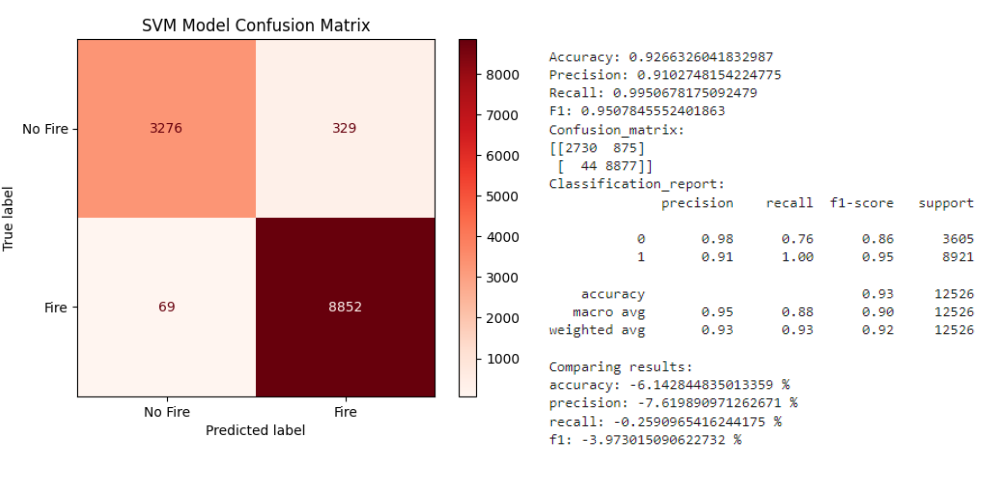
\includegraphics[width=0.75\linewidth]{images/SVM.png}
    \caption{SVM Metric}
    \label{fig: SVM Model}
\end{figure}

\begin{figure}
    \centering
    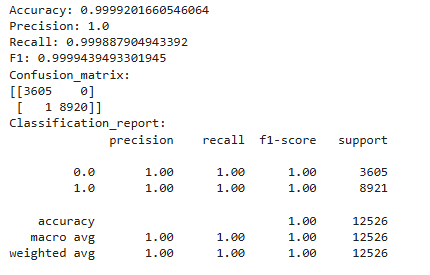
\includegraphics[width=0.75\linewidth]{images/12acc.png}
    \caption{12 - Feature Metrics}
    \label{fig: 1.0 }
\end{figure}

\begin{figure}
    \centering
    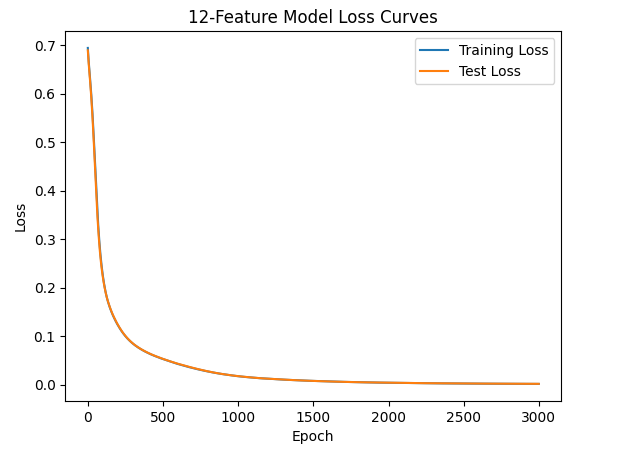
\includegraphics[width=0.75\linewidth]{images/12CM.png}
    \caption{12 - Feature Loss Curve}
    \label{fig: 1.2}
\end{figure}

\begin{figure}
    \centering
    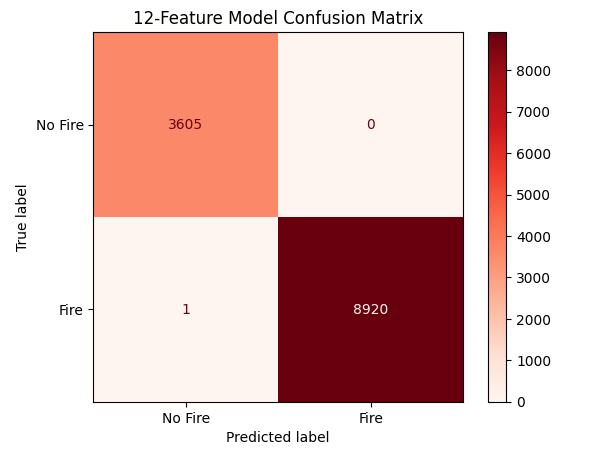
\includegraphics[width=0.75\linewidth]{images/12CMM.png}
    \caption{12 - Feature Confusion Matrix}
    \label{fig:1.3}
\end{figure}

\begin{figure}
    \centering
    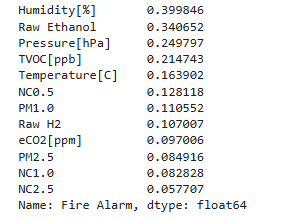
\includegraphics[width=0.7\linewidth]{images/Corr.png}
    \caption{Features}
    \label{fig:2.0-label}
\end{figure}

\begin{figure}
    \centering
    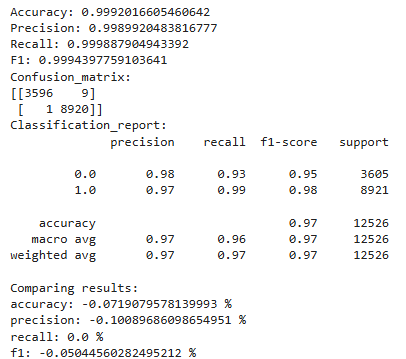
\includegraphics[width=0.75\linewidth]{images/4metric.png}
    \caption{4 - Feature Metrics}
    \label{fig:3.0}
\end{figure}

\begin{figure}
    \centering
    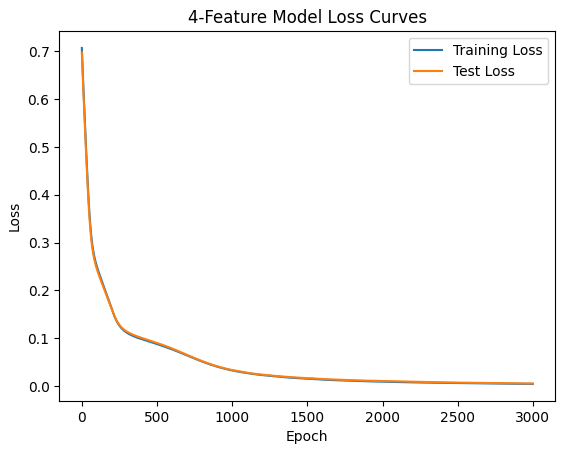
\includegraphics[width=0.75\linewidth]{images/4LC.png}
    \caption{4 - Feature Loss Curves}
    \label{fig:3.1}
\end{figure}

\begin{figure}
    \centering
    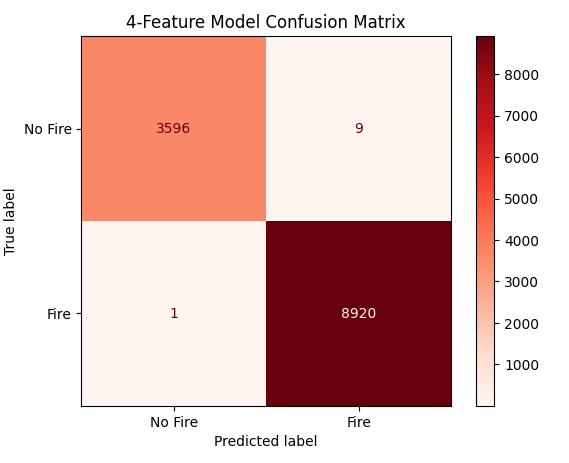
\includegraphics[width=0.75\linewidth]{images/4CM.png}
    \caption{4 - Feature Confusion Matrix}
    \label{fig:3.2}
\end{figure}

\begin{figure}
    \centering
    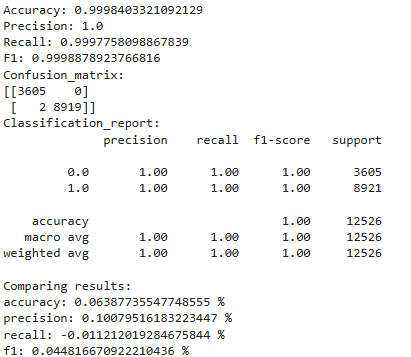
\includegraphics[width=0.75\linewidth]{images/5metric.png}
    \caption{5 - Feature Metrics}
    \label{fig:4.0}
\end{figure}

\begin{figure}
    \centering
    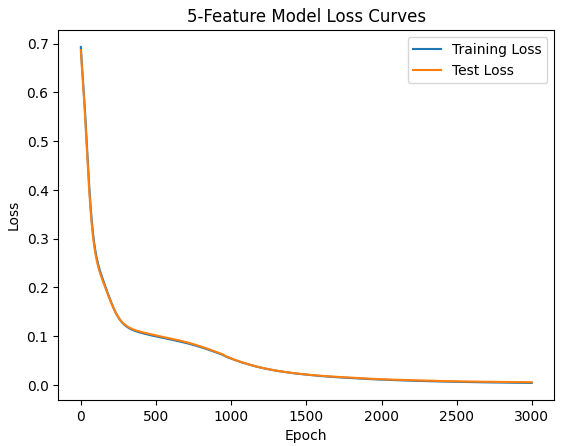
\includegraphics[width=0.75\linewidth]{images/5LC.png}
    \caption{5 - Feature Loss Curves}
    \label{fig:4.1}
\end{figure}

\begin{figure}
    \centering
    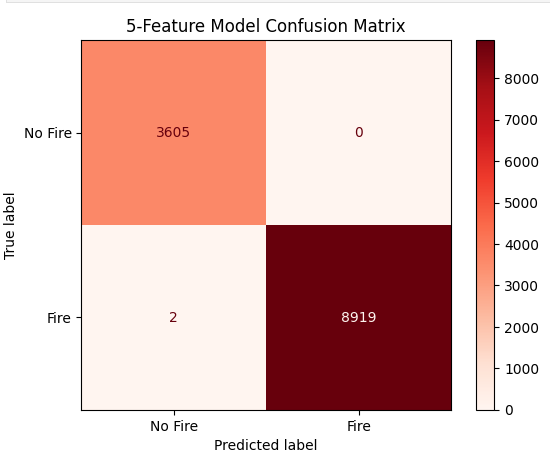
\includegraphics[width=0.75\linewidth]{images/5CM.png}
    \caption{5 - Feature Confusion Matrix}
    \label{fig:4.2}
\end{figure}

\begin{figure}
    \centering
    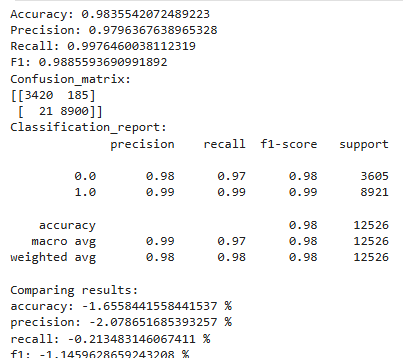
\includegraphics[width=0.75\linewidth]{images/imputationmetric.png}
    \caption{Imputation Metrics}
    \label{fig:5.0}
\end{figure}
\begin{figure}
    \centering
    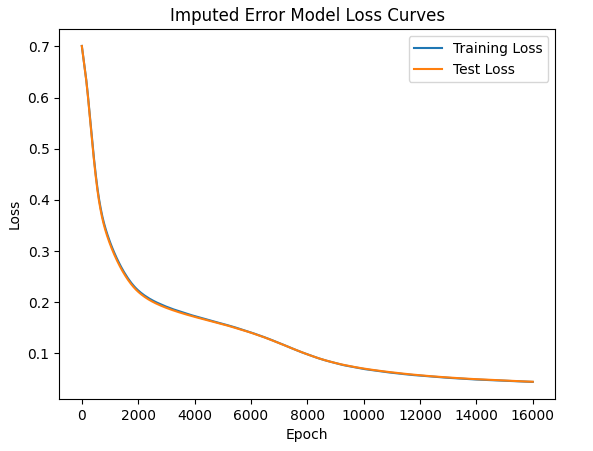
\includegraphics[width=0.75\linewidth]{images/ImputationLC.png}
    \caption{Imputation Loss Curves}
    \label{fig:5.1}
\end{figure}

\begin{figure}
    \centering
    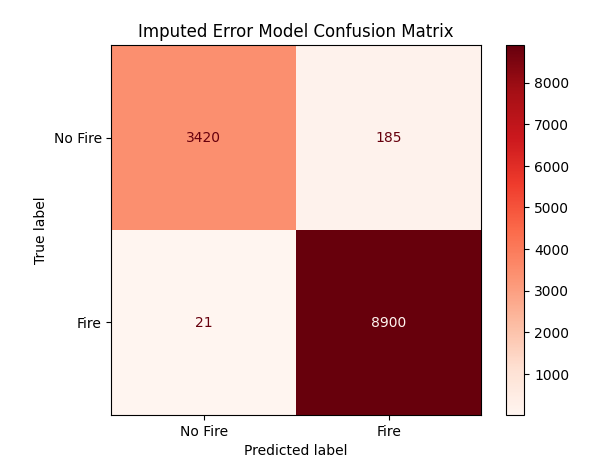
\includegraphics[width=0.75\linewidth]{images/ImputationCM.png}
    \caption{Imputation Confusion Matrix}
    \label{fig:5.2}
\end{figure}


\begin{figure}
    \centering
    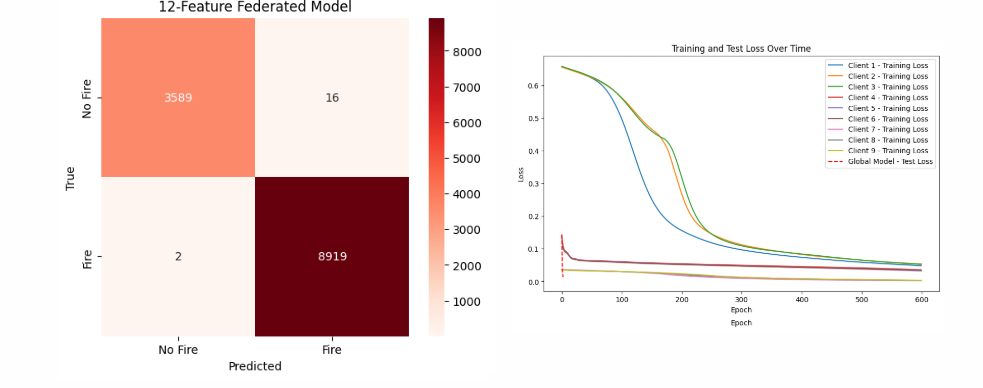
\includegraphics[width=1\linewidth]{images/12Fed.png}
    \caption{Federarted Learning: 12-Features}
    \label{fig:6.0}
\end{figure}

\begin{figure}
    \centering
    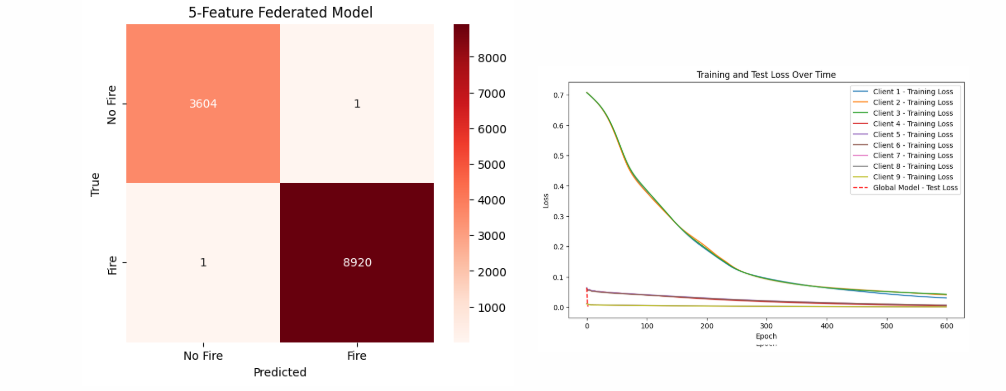
\includegraphics[width=1\linewidth]{images/5Fed.png}
    \caption{Federated Learning: 5-Features}
    \label{fig:6.1}
\end{figure}

\begin{figure}
    \centering
    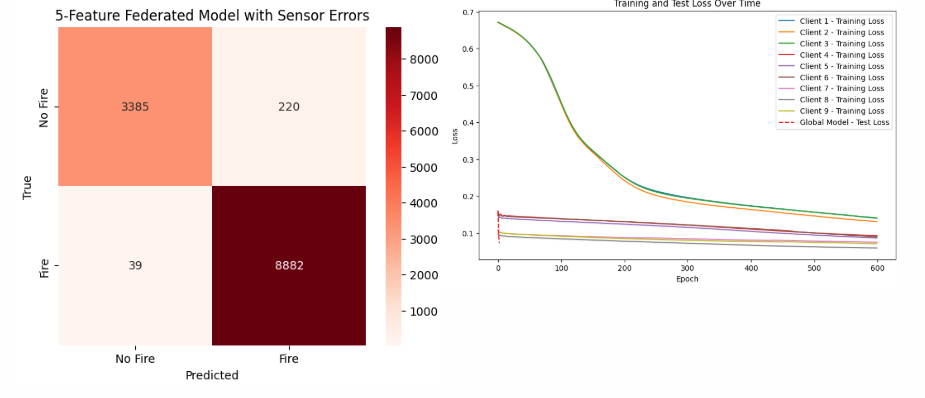
\includegraphics[width=1\linewidth]{images/FedHandling.png}
    \caption{Federated Learning: Error handling}
    \label{fig:6.2}
\end{figure}

\begin{figure}
    \centering
    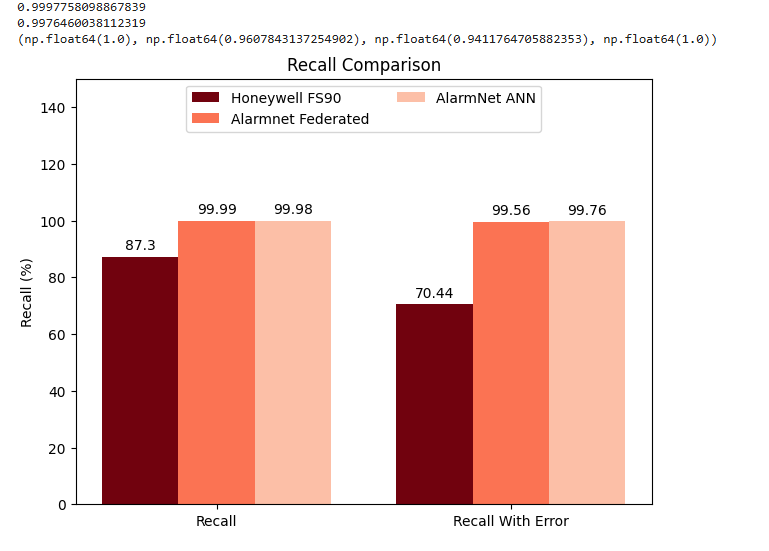
\includegraphics[width=0.75\linewidth]{images/Recall.png}
    \caption{Recall Comparison Honeywell FS90 Vs AlarmNet ANN Vs Federated}
    \label{fig:7.0}
\end{figure}

\begin{figure}
    \centering
    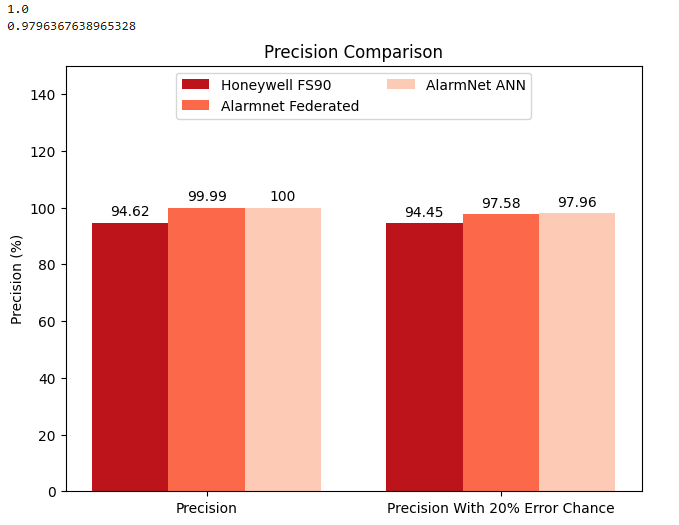
\includegraphics[width=0.75\linewidth]{images/PrecisionComparison.png}
    \caption{Precison Comparison Honeywell FS90 Vs AlarmNet ANN Vs Federated}
    \label{fig:7.1}
\end{figure}

\end{document}